\chapter{Mathematical Formulation}\label{chap:Math_for}
This chapter introduces the mathematical formulation of algorithms utilized in the power system, including the component modeling of the grid, power flow calculation, and state estimation algorithms. The IEEE European Low Voltage system with 206 nodes, which is a purely radial network, is presented and tested in this thesis. To simplify the problem, the distribution grid in our case is assumed to be balanced and the single phase equivalent model is used. The four estimators which will be tested on the distribution grid are explained in detail.

\section{Grid Model And Measurement Model }\label{subsec:power_flow}
To monitor the condition of the distribution grid, the DMS needs to collect information about the operational state and topology of the grid. Those data is imported into the state estimator to identify the state of the system and further actions could be made based on the state of the system. With the help of Geospatial Information System (GIS) and various sensors, the position of the tap changer, breaker's state, line connections and shunt capacitors can be known. Knowing the system topology and the injection at each bus, power flow calculation is run to calculate the flow through the distribution lines. Assuming that the system is balanced, a two-port $\pi$ model is used for representing the branch between two nodes in the distribution grid as shown in Fig.~\ref{fig:Line_model}.
    \begin{figure}[!h]
        \centering
        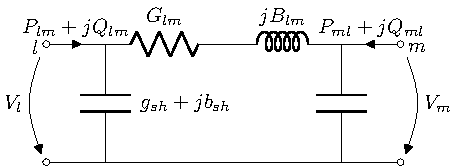
\includegraphics{figures/Line_model.pdf}
            \caption{Two-port $\pi$ model of a branch in distribution grid \cite{gomez2004power}}
        \label{fig:Line_model}
    \end{figure}
\bigskip

\subsection{Measurement Function} \label{subsec:h}

The measurement function $h(x)$ is a function which maps the estimated state of the system to the actual measurements. The most commonly used measurements are the line power flows, bus power injections, and bus voltage magnitudes. With the definition of the state of the system in introduced in Sect.~\ref{subsec:state_estimation}, the measurement function $h(x)$ can be written as follows:
    \begin{align} 
    h(x) &=      
        \begin{bmatrix}
            h^V(x)\\[6pt]
            h^{P_{inj}}(x)\\[6pt]
            h^{Q_{inj}}(x)\\[6pt]
            h^{P_{flow}}(x)\\[6pt]        
            h^{Q_{flow}}(x)         
        \end{bmatrix}
        =
        \begin{bmatrix}
            V_{mag}\\[6pt]
            P_{inj}\\[6pt]
            Q_{inj}\\[6pt]
            P_{flow}\\[6pt]        
            Q_{flow}         
        \end{bmatrix}
	    \label{eq:measurement_function}
    \end{align} 
Given the state of the system $x$, the elements in the measurement function can be formulated as follows:
\begin{itemize}
    \item $h^V(x)$ maps the state of the system to the voltage magnitude:
    \begin{align}
        h^V(x) &= V_{mag}
    \end{align}
    \item $h^{P_{inj}}$ and $h^{Q_{inj}}$ maps the state of the system to the real and reactive power injection ,respectively. For example, the active power injection $P_l$ and the reactive power injection $Q_l$ at bus $l$ can be formulated as:
        \begin{align} 
    	    h^{P_{l}} &= P_{l} 
    	    = V_{l} \sum_{m \in N_l}V_{m} \left(G_{lm}\cos{\theta_{lm}} + B_{lm}\sin{\theta_{lm}} \right)
    	    \label{eq:Pinj} \\[1pt]
    	    h^{Q_{l}} &= Q_{l} = V_{l} \sum_{m \in N_l}V_{m} \left(G_{lm}\sin{\theta_{lm}} - B_{lm}\cos{\theta_{lm}} \right)
    	    \label{eq:Qinj}
        \end{align}
    \item $h^{P_{inj}}$ and $h^{Q_{inj}}$ maps the state of the system to the active power flow and reactive power flow ,respectively. For example, the active power flow $P_{lm}$ and the reactive power flow $Q_{lm}$ from bus $l$ to bus $m$ equals to:
        \begin{align} 
    	    h^{P_{lm}} &= P_{lm} = V_{l}^2 \left(G_{lm}+g_{sh} \right)-V_{l}V_{m}\left(G_{lm}\cos{\theta_{lm}} + B_{lm}\sin{\theta_{lm}} \right)
    	    \label{eq:flow_active} \\[1pt]
    	    h^{Q_{lm}} &= Q_{lm} = -V_{l}^2 \left(B_{lm}+b_{sh} \right)-V_{l}V_{m}\left(G_{lm}\sin{\theta_{lm}} - B_{lm}\cos{\theta_{lm}} \right)
    	    \label{eq:flow_reactive}
        \end{align}    
\end{itemize}
, where
$G_{lm} + jB_{lm}$ is the admittance of the branch connected between bus $l$ and bus $m$ and $g_{sh} + jb_{sh}$ is the shunt admittance of the branch connected at bus $l$ or bus $m$ as shown in Fig.~\ref{fig:Line_model}. $N_{l}$ is the set of buses connected to bus $l$. $V_l$ and $V_m$ are the voltage magnitudes at bus $l$ and bus $m$ respectively, and $\theta_{lm}$ represents the phase difference between bus $l$ and bus $m$ \cite{gomez2004power}. 
\bigskip
\\Equations \ref{eq:Pinj} to \ref{eq:flow_reactive} contain the four following variables: active power $P$, reactive power $Q$, voltage magnitude $V$ and phase $\theta$. The above equations show that, under the assumption that all the parameters of the system, such as the impedance of the branches, tap position of the transformer and state of the breakers, and at least two of the four variables are known, the remaining variables can be calculated. Those equations are utilized for both power flow calculation and measurement function in state estimation, and are physical laws that need to be fulfilled. The most typical method for solving the above equations is the Newton-Raphson method (NR) which is used in this project. As mentioned, the above equations are also part of measurement function $h(x)$, which calculate the branch power flow and bus power injection based on the state $x$. In conclusion, the measurement function $h(x)$ can map the state of the system to its bus voltage magnitudes, bus power injection, and power flow, notably measured by the smart meters, based on Equations \ref{eq:Pinj} to \ref{eq:flow_reactive}.

\subsection{Measurement Jacobian Matrix} \label{jacobian_matrix}
The measurement Jacobian matrix $H$ is defined as the first-order partial derivative of the measurement matrix $h$ with respects to the state of the system: 
\bigskip
\begin{align} 
    H(x) &= \frac{\partial h(x)}{\partial x} 
    =      
    \begin{bmatrix}
                \frac{\partial V_{mag}}{\partial \theta} & \frac{\partial V_{mag}}{\partial V} \\[6pt]
                \frac{\partial P_{inj}}{\partial \theta} & \frac{\partial P_{inj}}{\partial V} \\[6pt]
                \frac{\partial Q_{inj}}{\partial \theta} & \frac{\partial Q_{inj}}{\partial V} \\[6pt]
                \frac{\partial P_{flow}}{\partial \theta} & \frac{\partial P_{flow}}{\partial V} \\[6pt]        \frac{\partial Q_{flow}}{\partial \theta} & \frac{\partial Q_{flow}}{\partial V}             
            \end{bmatrix}
    \label{eq:jacobian_matrix} 
\end{align}
The measurement Jacobian matrix has $m$ rows and $n$ columns, where $m$ equals to the number of measurements and $n$ equals to the number of states. To be more specific, the components in the measurement Jacobian matrix can be written as follows \cite{jaman2017implementation}:
\begin{itemize}
    \item The partial derivative of the voltage magnitude can be formulated as:
        \begin{align} 
    	    \frac{\partial V_{mag}}{\partial \theta} &= 0
    	    \label{eq:V_mag_theta} \\[1pt]
    	    \frac{\partial V_{l}}{\partial V_{l}} &= 1
    	    \label{eq:V_mag_l} \\[1pt]
    	    \frac{\partial V_{l}}{\partial V_{m}} &= 0 
    	    \label{eq:V_mag_m} 
        \end{align}
    \item The components of the measurement Jacobian matrix corresponding to active power injection can be expressed as:
        \begin{align} 
    	    \frac{\partial P_{l}}{\partial \theta_l} &= \sum_{m=1}^{N}V_l V_m \left(-G_{lm}\sin{\theta_{lm}}+B_{lm}\cos{\theta_{lm}}\right)-V_l^2 B_{ll}
    	    \label{eq:P_inj_theta_l} \\[1pt]
    	    \frac{\partial P_{l}}{\partial \theta_m} &= V_l V_m \left(G_{lm}\cos{\theta_{lm}}-B_{lm}\sin{\theta_{lm}}\right)
    	    \label{eq:P_inj_theta_m} \\[1pt]
    	    \frac{\partial P_{l}}{\partial V_l} &= \sum_{m=1}^{N}V_m \left(G_{lm}\cos{\theta_{lm}}+B_{lm}\sin{\theta_{lm}}\right)-V_l^2 G_{ll} \\[1pt]
    	    \label{eq:P_inj_V_l}
            \frac{\partial P_{l}}{\partial V_m} &= V_l \left(G_{lm}\cos\theta_{lm}+B_{lm}\sin\theta_{lm} \right) 
    	    \label{eq:P_inj_theta_m}     	    
        \end{align}    
    \item The components of the measurement Jacobian matrix related to the reactive power injection can be derived as:
        \begin{align} 
    	    \frac{\partial Q_{l}}{\partial \theta_l} &= \sum_{m=1}^{N}V_l V_m \left(G_{lm}\cos{\theta_{lm}}+B_{lm}\sin{\theta_{lm}}\right)-V_l^2 B_{ll}
    	    \label{eq:Q_inj_theta_l} \\[1pt]
    	    \frac{\partial Q_{l}}{\partial \theta_m} &= V_l V_m \left(-G_{lm}\cos{\theta_{lm}}-B_{lm}\sin{\theta_{lm}}\right)
    	    \label{eq:Q_inj_theta_m} \\[1pt]
    	    \frac{\partial Q_{l}}{\partial V_l} &= \sum_{m=1}^{N}V_m \left(G_{lm}\sin{\theta_{lm}}-B_{lm}\cos{\theta_{lm}}\right)-V_l^2 G_{ll} \\[1pt]
    	    \label{eq:Q_inj_V_l}
            \frac{\partial Q_{l}}{\partial V_m} &= V_l \left(G_{lm}\sin\theta_{lm}-B_{lm}\cos\theta_{lm} \right) 
    	    \label{eq:Q_inj_theta_m}     	    
        \end{align}
    \item As for the measurement Jacobian matrix entries related to the active power flow on the branches:
        \begin{align} 
    	    \frac{\partial P_{lm}}{\partial \theta_l} &= V_l V_m \left(g_{lm}\sin{\theta_{lm}}-b_{lm}\cos{\theta_{lm}}\right)
   	        \label{eq:P_lm_theta_l} \\[1pt]
       	    \frac{\partial P_{lm}}{\partial \theta_m} &= -V_l V_m \left(g_{lm}\sin{\theta_{lm}}-b_{lm}\cos{\theta_{lm}}\right)
   	        \label{eq:P_lm_theta_m} \\[1pt]
       	    \frac{\partial P_{lm}}{\partial V_l} &= -V_m \left(g_{lm}\cos{\theta_{lm}}+b_{lm}\sin{\theta_{lm}}\right)+2\left(g_{lm}+jg_{sh} \right)V_l
   	        \label{eq:P_lm_V_l} \\[1pt]
      	    \frac{\partial P_{lm}}{\partial V_m} &= -V_l \left(g_{lm}\cos{\theta_{lm}}+b_{lm}\sin{\theta_{lm}}\right)
   	        \label{eq:P_lm_V_m}
        \end{align}        
    \item Elements representing the partial derivative of the reactive power flow with respective to the states:
        \begin{align} 
    	    \frac{\partial Q_{lm}}{\partial \theta_l} &= V_l V_m \left(g_{lm}\cos{\theta_{lm}}+b_{lm}\sin{\theta_{lm}}\right)
   	        \label{eq:Q_lm_theta_l} \\[1pt]
       	    \frac{\partial Q_{lm}}{\partial \theta_m} &= V_l V_m \left(g_{lm}\cos{\theta_{lm}}+b_{lm}\sin{\theta_{lm}}\right)
   	        \label{eq:Q_lm_theta_m} \\[1pt]
       	    \frac{\partial Q_{lm}}{\partial V_l} &= -V_m \left(g_{lm}\sin{\theta_{lm}}-b_{lm}\cos{\theta_{lm}}\right)-2\left(b_{lm}+jb_{sh} \right)V_l
   	        \label{eq:Q_lm_V_l} \\[1pt]
      	    \frac{\partial Q_{lm}}{\partial V_m} &= -V_l \left(g_{lm}\sin{\theta_{lm}}+b_{lm}\cos{\theta_{lm}}\right)
   	        \label{eq:Q_lm_V_m}
        \end{align}     
    
\end{itemize}
\\With the help of the equations above, the measurement Jacobian matrix can be derived once the topology and the input voltages are determined. Notice that the measurement Jacobian matrix does not change significantly with respect to the input voltage magnitude and phase due to the fact that the p.u. value of the input voltages are close to the flat start. This means that whose voltage magnitudes are close to 1 p.u. and voltage phases are close to zero. By knowing this property of the measurement Jacobian matrix, the computational burden burden can be relaxed by calculating the measurement Jacobian matrix just once at the beginning with a flat start input.

\section{State Estimation Algorithms} \label{subsec:state_estimation}
In this section, the mathematical formulation of four state estimation algorithms, namely WLS, EKF, SHGM, and SVR-EKF will be introduced. All these algorithms except SVR-EKF have already been widely implemented and tested both in simulations and real transmission grid, and the results show that all of them are robust and efficient in the transmission grid. In this thesis they are tested in the low voltage distribution grid and the performance of these algorithms is compared.
\bigskip
\\State estimation is one of the most important functions in EMS. With the help of the great number of measurement devices in transmission grid or pseudo-measurements in the distribution grid, high redundancy can be obtained. This requires state estimation to estimate the most likely state of the system based on noisy, faulty or inaccurate measurements and pseudo-measurements. There are totally three type of measurements in this thesis, including: 
\begin{itemize}
    \item Real measurements from the smart meters which are subject to noise as stated above. The noise of the measurements are determined by the precision of the measurement devices and the surrounding situation. 
    \item Pseudo-measurements are not real measurements but an estimation of the actual value to ensure the observability of the system. Per definition, these are substantially less accurate than real measurements. Details about how to generate pseudo-measurements will be introduced further.
    \item  Virtual measurements are derived from the status of grid components. For example, when there is no load or generator connected to one bus, then the power injection at this bus can be set to zero. If this bus is at the end of one branch, then the power flow across this branch is also zero. To simplify the problem, only the power injection at the buses without load and generator are be treated as virtual buses and the power flow of branches is not considered. This kind of measurements should have higher precision than the real and pseudo-measurements, but for the sake of simplicity, real and virtual measurements are assumed to have the same precision in this thesis.
\end{itemize}
\bigskip
\\With the help of the above measurements, the most likely state of the system is estimated in the DMS. Typically, the state estimator has the following functions
\cite{gomez2004power}: 
\begin{itemize}
    \item Topology processor: Determine the topology of the system and build the single phase or three-phase diagram based on the collected data about the status of circuit breakers and switches.
    \item Observability check: Identify the observability of the system based on the existing measurements. If the system is unobservable, the unobservable lines and observable islands should be identified.
    \item State estimation: Find the optimal state of the system by minimizing the difference between the estimated value and the measurements. The state of the system is defined as the voltage magnitude and phase of each bus. And bus one is defined as the slack bus whose phase is set to zero and assumed to be known in advance. For example, the state $x$ of a system with $N$ number of buses is:
        \begin{align} 
    	    x &=  [\theta_{2} \quad \theta_{3} \quad \cdots \quad \theta_{N} \quad V_{1} \quad V_{2} \quad \cdots \quad V_{N} ]^\intercal
    	    \label{eq:state} 
        \end{align}
   
    \item Bad data processing: Firstly, the bad data detection should be executed among the measurements. Bad data are either eliminated or corrected. However, bad data detection and identification are not investigated in this thesis. The main reason is that there is a great proportion of pseudo-measurements across all measurements to allow the system to be observable. All these pseudo-measurements are very likely to be detected as bad data, and the system is not observable if all these pseudo-measurements are eliminated.
    \item Parameter and structure error processing: Detect the possible parameter and structure errors of the system such as the branches connection error and inaccurate line impedance.
\end{itemize}
\bigskip
\\After estimating the state of the system, the measurements $z$ of the system can be uniquely calculated based on the measurement function $h(x)$ which maps the state x to the measurements z as shown in ~Equation \ref{eq:meas_fun}:
    \begin{align} 
        z &=  \begin{bmatrix}
                    z_{1} \\
                    z_{2} \\
                    \vdots \\
                    z_{m} \\
              \end{bmatrix}
          = \begin{bmatrix}
                    h_1(x) \\
                    h_2(x) \\
                    \vdots \\
                    h_m(x) \\
              \end{bmatrix} +
            \begin{bmatrix}
                    e_1 \\
                    e_2 \\
                    \vdots \\
                    e_m \\
              \end{bmatrix}  
          = h(x)+e
        \label{eq:meas_fun}
    \end{align}
\\, where:    
\begin{itemize}
    \item $z$ is the measurements vector with $m$ number of measurements.
    \item $h_i(x)$ is the non-linear measurement function which maps the state vector $x$ to $i^{th}$ measurement $z_i$. 
    \item $h(x)=\begin{bmatrix}
                    h_{1}(x) &
                    h_{2}(x) &
                    \cdots &
                    h_{m}(x) 
              \end{bmatrix}^\intercal$ 
    \item $e=\begin{bmatrix}
                e_{1} &
                e_{2} &
                \cdots &
                e_{m} 
          \end{bmatrix}^\intercal$.          
    \item $e_{i}$ represents the error between the real value of measurement $h_{1}(x)$ and the measurement from the meter $z_i$ due to the limited accuracy of the meter, a faulty measurement or a pseudo-measurement
    \end{itemize}
    \\The error from meters is assumed to be a white Gaussian noise with zero mean $\mu_{noise}$ and standard deviation $\sigma$. As a result, the error should have the following statistic properties\cite{gomez2004power}:
    \begin{itemize}
        \item Expected value $E(e_i)=\mu_{noise}$ for $i=1,2,...m$.
        \item The errors of each measurement are independent from each other, which means $E(e_i e_j)=0$ for $i=1,2,...m$, $j=1,2,...m$. Thus, the covariance matrix is $R=Cov(e)=E(e\cdot e^\intercal)=diag \big\{ \sigma_{1}^2, \sigma_{1}^2, \cdots, \sigma_{m}^2\big\}$ which reflect the accuracy of measurements.
    \end{itemize}  
\\Based on the assumptions above, the normal probability density function of the measurement vector $z$ can be written as:
\begin{align}
    f\left(z \right) &= \frac{1}{\sqrt{2\pi}\sigma}e^{-\frac{1}{2}\left(\frac{z-\mu}{\sigma}\right)^2}
    \label{eq:pro_den_fun}
\end{align}
, where
\begin{itemize}
    \item $\mu$ is the expected value of the measurement.
    \item $\sigma$ is the standard deviation of the measurement $z$.

\end{itemize}


\subsection{Weigted Least Squares}
\\Weighted Least Squares (WLS) is currently the most widely used state estimation algorithm in the transmission grid due to its high robustness and low computational burden. The object of WLS to obtain the most likely state of the system or to minimize the sum of the weighted squares of the residual $r$, which is defined as the difference between the estimated measurements and the actual measurements from the meters:
\begin{align}
    r &= z-h(x)
    \label{eq:residual}
\end{align}
\subsubsection{Objective Function Formulation}
\\Considering that the normal probability density function of measurements are independent from each other, the joint probability density function of the system with $m$ measurements can be written as:
\begin{align}
    f_m(z) &= f(z_1)f(z_2) \cdots f(z_m)
    \label{eq:likelihood}
\end{align}
,where $f_m(z)$ is the probability density function of the $m$ measurements which shows the probability of the system to be at the state $z$. And the goal is to maximize $f_m(z)$ by tuning the variable $\mu$ and $\sigma$ stated in Equation \ref{eq:pro_den_fun}. Before solving the objective function, a modification is applied to Equation \ref{eq:likelihood} by adding a logarithm ahead of the equation, which is called Log-Likelihood function $\mathcal{L}$:
\begin{align}
    \mathcal{L} &=\log f_m(z) 
    = -\frac{1}{2} \sum_{i=1}^{m} \left(\frac{z_i-\mu_i}{\sigma_i} \right)^2-\frac{m}{2}\log 2\pi- \sum_{i=1}^{m} \log \sigma_i
    \label{eq:log_likelihood}
\end{align}
In Equation \ref{eq:log_likelihood}, the last two elements are constant values which can be neglect, together with the constant factor ahead of the first element, when solving the optimization problem. Hence, the new objective function $J$ can be re-written as:
\begin{equation}
    \begin{aligned}
    & \underset{x}{\text{minimize}}
    & & J(x)=\sum_{i=1}^{m} W_{ii} {r_i} ^2 \\
    & \text{subject to}
    & & r_i = z_i-h_i(x), \; i = 1, \ldots, m.\\
    \label{eq:obj_fun_WLS}
    \end{aligned}
\end{equation}
, where $W_{ii}=\frac{1}{\sigma_{i}^2}$ is $i_{th}$ element of the diagonal weight matrix $W$.   

\subsubsection{Solution of WLS}
\\To find the solution of Equation \ref{eq:obj_fun_WLS}, the first-order optimality condition is sufficient to satisfy the minimization problem \cite{gomez2004power}:
\begin{align}
    g(x) &= \frac{\partial J(x)}{\partial x} 
          = -H^\intercal(x) W (z-h(x))
          =0
    \label{eq:min_der_WLS}      
\end{align}
\\, where $H$ is the measurement Jacobian matrix defined in Equation \ref{eq:jacobian_matrix}. To solve non-linear Equation \ref{eq:min_der_WLS}, Taylor series expansion is applied around the variable $x^k$:
\begin{align}
    g(x) &= g(x^k)+G(x^k)(x-x^k)+\cdots =0
    \label{eq:tyalor_series_g}
\end{align}
, where $G(x^k)$ is called the Gain matrix and formulated as:
\begin{align}
    G(x^k) &= \frac{\partial g(x^k)}{\partial x}
    =H^\intercal(x^k) W H(x^k )
    \label{eq:gain_matrix}
\end{align}
After neglecting the higher order elements in Equation \ref{eq:tyalor_series_g}, the equation goes into a form which can be solved with Gauss-Newton algorithm for minimizing the cost function iteratively:
\begin{align}
     \Delta x^{k+1} &= -[G(x^k)]^{-1} g(x^k)
    \label{eq:WLS_GN}
\end{align}
, where:
\begin{align}
     \Delta x^{k+1} &= x^{k+1}-x^k
    \label{eq:delta_x}
\end{align}
The iteration can be stopped when $\Delta x^{k+1}$ is smaller than a predetermined threshold or the iteration number exceeds a certain number. Because both the measurement Jacobian matrix $H$ and Gain matrix are usually sparse, the Gain matrix $G$ in Equation \ref{eq:WLS_GN} can be ill-conditioned and not invertible. As a result, matrix decomposition skills are utilized to solve Equation \ref{eq:WLS_GN} in a more robust and fast way. Cholesky decomposition is used in this project for solving the equations which contain the inverse of Gain matrix \cite{gomez2004power}. 

\subsection{Extended Kalman Filter}
\label{sect:EKF}
\\In order to make use of the availability of the historical data during state estimation, Dynamic State Estimation (DSE) algorithms are developed for improving the accuracy of the estimator by considering both the real-time data and prediction based on the historical data. Kalman Filter techniques are introduced into state estimation for enhancing the performance of the traditional WLS. There are two typical algorithms proposed with Kalman Filter, Extended Kalman Filter (EKF) \cite{jaman2017implementation} and Unscented Kalman Filter (UKF) \cite{valverde2011unscented}. In this project, EKF is selected as the tested DSE algorithm which includes three main steps of parameter identification, state forecasting, and state correction. EKF is preferred over UKF in this thesis since it has a lower computational burden on Matlab.
\bigskip
\\Assuming the system is operated under quasi steady-state condition, the behavior function of the system can be described as:
\begin{align}
    x_{t+1} &= F_t x_t + g_t +u_t
    \label{eq:quasi_steady_state behaviour function}
\end{align}
, where $t$ is the time sample, $x$ is the state vector, $F_t$ represents the state transition function, vector $g_t$ is associated with the behavior trends of the state trajectory and vector $u_t$ denotes the uncertainty with zero mean and covariance matrix $Q_t$.

\subsubsection{Parameter Identification}
During the first step before forecasting, the values of parameters $F_t$, $g_t$ and $q_t$ should be determined. The white Gaussian noise uncertainty matrix is adjusted by the user, in this project the diagonal elements of the uncertainty matrix are set to 10. In addition, Holt's linear exponential smoothing technique is applied to calculate $F_t$, $g_t$, which is a simple method for short-term time series prediction \cite{da1983state}. The advantage of this forecasting method is that only a small number of historical time step data is used for prediction which reduces the computational burden. To be more specific, these two parameters can be calculated as:
\begin{align}
    F_t &= \alpha_t (1+ \beta_t) I 
    \label{eq:quasi-transition matrix}\\[1pt]
    g_t &= (1+\beta_t)(1-\alpha_t)\widetilde{x}_t-\beta_t a_{t-1} + (1-\beta_t)b_{t-1}
    \label{eq:behaviour_trend matrix}
\end{align}
, where $\alpha_t$ and $\beta_t$ are smoothing parameters at time step $t$ lying between 0 and 1, and they should also satisfy the condition $\alpha_t$ > $\beta_t$. In this project, these two parameters are set to 0.97 and 0.02 for all time steps, respectively. $I$ represents the identity matrix and $\widetilde{x}_t$ means the forecast state at time step $t$. Parameters $a_t$ and $b_t$ are the level and trend at time step $t$, where level index gives an estimate of the local mean and trend represents the change between two successive time steps. They can be obtained by the following equations:
\begin{align}
    a_t &= \alpha_t \hat{x}_t + (1-\alpha_t) \widetilde{x}_t 
    \label{eq:EKF_parameter_a}\\[1pt]
    b_t &= \beta_t (a_t - a_{t-1})+(1-\beta_t)b_{t-1}
    \label{eq:EKF_parameter_b}
\end{align}
, where $\hat{x}_t$ is the estimated state value at time step $t$. With the help of the above equations, the state of the system at the next time step can be predicted.

\subsubsection{State Prediction}
\\After the parameter identification stage, the state of next time step $\widetilde{x}_t$ together with its covariance matrix $P_{\widetilde{x}_t}$ can be predicted:
\begin{align}
    \widetilde{x}_t &= F_t \hat{x}_t +g_t \label{eq:EKF_forecasting_state}
    \\[1pt]
    P_{\widetilde{x}_{t+1}} &= F_t P_{\hat{x}_t} F_t^\intercal +Q_t 
    \label{eq:EKF_forecasting_state_covariance_matrix}
\end{align}
, where $P_{\hat{x}_t}$ is the covariance matrix of predicted state $\hat{x}_t$ at time step $t$. It should be noticed that  $\hat{x}_t$ and $\widetilde{x}_t$ do not include the voltage phase at the feeder bus in Equation \ref{eq:EKF_forecasting_state} and is added after the prediction stage as 0.
\bigskip
 \\In the state estimation, the states which need to be predicted are the voltage phases and voltage magnitude. This forecasting method is more suitable for quasi-steady state. The performance of Holt's linear exponential smoothing technique is not satisfied when the state of the system changes significantly between each time step. In this case, some other forecasting techniques are derived such as Artificial Neural Network (ANN) and Support Vector Regression (SVR).

\subsubsection{State Correction}
In the state correction stage, the state of the system $\hat{x}_{t+1}$ should be estimated based on the measurement $z$ at time step $t+1$ and the forecasted state $\widetilde{x}_{t+1}$. The following objective function can be formulated to calculate the state vector:
\begin{align}
    J(\hat{x}_{t+1})=[z-h(\hat{x}_{t+1})]^\intercal W [z-h(\hat{x}_{t+1})] + (\hat{x}_{t+1}-\widetilde{x}_{t+1})^\intercal P^{-1}_{\widetilde{x}_{t+1}} (\hat{x}_{t+1}-\widetilde{x}_{t+1})
    \label{eq:EKF_objective_function}
\end{align}
Compared with the objective function of WLS in Equation \ref{eq:obj_fun_WLS}, the objective function of EKF considers the influence from both the measurement $z$ collected at time step $t+1$ and the prediction $\widetilde{x}_{t+1}$ made at time step $t$. To solve the minimization problem in Equation \ref{eq:EKF_objective_function}, the Taylor expansion method and first-order optimality condition can be applied similarly to WLS as follows:
\begin{align}
    x^{k+1} &= x^k +K_{t+1} (z-H_{t+1} \widetilde{x}_{t+1})
    \label{eq:EKF_first_order}
\end{align}
, where $K_{t+1}$ is the Kalman gain at time step $t$ defined as:
\begin{align}
    K_{t+1} &= P_t H_{t+1}^{\intercal} R^{-1}
    \label{eq:EKF_kalman_gain}
\end{align}
$k$ is the iteration number. In EKF algorithms, only one iteration is applied as a trade-off between the computational burden and the accuracy of the result. In this project, the weight matrix $W$ in Equation \ref{eq:EKF_kalman_gain} is calculated by Cholesky decomposition. As for the error covariance matrix $P_{\hat{x}_{t+1}}$ of the estimated state, it can be obtained by:
\begin{align}
    P_{\hat{x}_{t+1}} &= \left(H^\intercal R^{-1} H + P_{\widetilde{x}_{t+1}}^{-1} \right)^{-1}
    \label{eq:estimated_state_covraicne_matrix}
\end{align}
Note that EKF needs several time steps to converge if flat start is used as starting point, i.e. initial voltage magnitudes of one and angles of zero. To make EKF comparable with other algorithms by eliminating the influence of the inaccurate results during the converging time steps, the initial estimated voltage magnitude $\hat{V_1}$ and voltage phase $\hat{\theta}_1$ are set to be one and zero, respectively, but the forecasted voltage magnitude $\widetilde{V}_1$ and $\widetilde{\theta}_1$ is assumed to be a perfect value and the phase angle $\widetilde{\theta}_1$ is set to zero at the first time step. The covariance matrix $P_{\widetilde{x}_1}$ is assumed to be zero at the first time step \cite{jaman2017implementation}. 

\subsection{SHGM}
\\Schweppe-type GM-estimator with the Huber psi-function, abbreviated as SHGM, is an algorithm which adapts the weight matrix considering the influence from the leverage points. A leverage point represents a measurement which has a considerably high influence on the resulting estimated state. In the SHGM algorithm, the leverage points are found with the help of the projection statistics method first, and the weight of the bad leverage points in the cost function are reduced.

\subsubsection{Concepts of Leverage Points}
\\Based on the introduction above, leverage points in power system state estimation are measurements which have a stronger influence on the results compared to other measurements. Assuming each row of the measurement Jacobian matrix $H$ represents one point in a $n$ dimension space where $n$ is the number of states and each element in this row is one dimension, some of the rows $H_i$ in the measurement Jacobian matrix $H$ might lies far away from other rows of the measurement Jacobian matrix, and the corresponding measurements of $H_i$ have a stronger influence than other measurements. The influence of each measurement on the estimated result can be expressed as \cite{gomez2004power}:
\begin{align}
    \hat{z} &= \Lambda z
    \label{eq:hat_matrix_equation}
\end{align}
, where $\hat{z}$ and $z$ are estimated and actual measurements, respectively. $\Lambda$ is called the hat matrix and can be calculated as follows:
\begin{align}
    \Lambda &= H G^{-1} H^{\intercal} W 
    \label{eq:hat_matrix_defination}
\end{align}
, where $G$ is the gain matrix introduced in Equation \ref{eq:gain_matrix}. The value of the diagonal elements in the hat matrix goes from zero to one, and represents the distance of the corresponding row $H_i$ with other rows of measurement Jacobian matrix. When $G_{ii}$ close to one, $H_i$ is far from other rows and likely to be a leverage point. The difference between critical measurements and leverage points is that the system can still be observable when the leverage point is eliminated \cite{gomez2004power}. 
\bigskip
\\Typically, the leverage points are more correlated with the topology and parameter of the grid, the measurement is likely to be a leverage point under following conditions \cite{gomez2004power}:
\begin{itemize}
    \item An injection measurement at bus which is connected to a lot of branches.
    \item Power injection measurements at the bus whose connected branches have very different line impedance.
    \item Power flow measurements whose branch impedance significantly differs from other branches of the system.
    \item Power flow measurement on a branch with short and small reactance.
\end{itemize}
\\As stated before, leverage points have a high impact on the accuracy of an estimator. If the measurement associated with a leverage point is good, the accuracy of the estimator is enhanced. However, if the measurement associated with a leverage point is bad, it may wreck the performance of the estimator \cite{rousseeuw1993alternatives}. As a result, the goal of SHGM is to identify the bad leverage points and reduce their influence on the result by giving them a lower weight. 

\subsubsection{Identify Leverage Points}
\\As the leverage points are defined as outliers in the bulk of points cloud, the leverage points identification in state estimation enables to find the rows of the measurement Jacobian matrix which are far away from other rows. To find the outliers in the measurement Jacobian matrix $H$, the Mahalanobis Distance can be used. Having $m$ as the number of rows of measurement Jacobian matrix $H(x)$ and $\{ l_1,l_2,\cdots,l_m \}$ the normalized rows of $H(x)$ which are calculated as:
\begin{align}
    l &= \sqrt{R^{-1}} H(x)
    \label{eq:normalized jacobian matrix l}
\end{align}
The Mahalanobis Distances of $l_i$ with respect to the rest of the rows is definded as:
\begin{align}
    MD_i &= \sqrt{(l_i-\bar{l})C^{-1}(l_i-\bar{l})}
    \label{eq:Mahalanobis distance}
\end{align}
, where $\bar{l}$ is the center of the normalized rows of measurement Jacobian matrix:
\begin{align}
    \bar{l} &= \frac{1}{m} \sum_{i=1}^{m} l_i
    \label{eq:center of l}
\end{align}
And $C$ is the covariance matrix of $l$ and is calculated as follows:
\begin{align}
    C &= \frac{1}{m-1} \sum_{i=1}^{m} (l_i-\bar{l}) (l_i-\bar{l})^\intercal 
    \label{eq:covar of l}
\end{align}
Assuming $l_i$ are Gaussian distributed, then $MD$ in Equation \ref{eq:Mahalanobis distance} follows a chi-square distribution where a threshold can be determined for identifying leverage points in $MD$. Rousseeuw and Croux proposed a new estimator for increasing the robustness and accuracy, which is called projection statistics \cite{rousseeuw1993alternatives}, and Mili applied the projection statistics method to power system state estimation for identifying the leverage points \cite{mili1996robust}. Projection statistics in state estimation is defined as:
\begin{align}
    PS_i &= \max _{v} \frac{|l_i^{\intercal}v|}{S_m}
    \label{eq:projection statistics}
\end{align}
, where $v=l_j, j=1,...,m$. $S_m$ is a scale estimator which represents the sample standard deviation of the projections of data points $l_i$ on the direction of vector $v$ proposed by Rousseeuw and Croux in \cite{croux1992time} and can be written as follows:
\begin{align}
    S_m &= 1.1926\{\underset{i}{lomed} (\underset{j \neq i}{lomed}| l_{i}^{\intercal}v + l_{j}^{\intercal}v|)\}f_m
    \label{eq:SHGM_Sm}
\end{align}
In Equation \ref{eq:SHGM_Sm}, $lomed$ means the low median of a series of elements and $f_m$ is a sample correction factor introduced in \cite{croux1992time}. This factor can make the scale estimator $S_m$ unbiased and its value is related to the number of measurements. When the number of measurements $m$ is smaller than 9 or even, $f_m$ is 1, otherwise when $m$ is larger than 9 and odd \cite{rousseeuw1993alternatives}:
\begin{align}
    f_m &= \frac{m}{m-0.9}
    \label{eq:SHGM fm}
\end{align}
Note that the nominator in Equation \ref{eq:projection statistics} can sometimes be equal to zero due to the sparsity of measurement Jacobian matrix which leads $PS$ to be infinity. To avoid this problem, the zero elements in $| l_{i}^{\intercal}v + l_{j}^{\intercal}v|$ should be eliminated when calculating the low median value in Equation \ref{eq:SHGM_Sm}.

\subsubsection{Algorithm of SHGM}
\\The first step of SHGM algorithm is the leverage points identification. Because leverage points are mainly related to the topology and parameters of the grid, this process can be achieved as an offline algorithm as long as the topology and parameter of the grid are unchanged. So, a flat start is used when calculating $H$ matrix. After that, the projection statistics $PS$ for each measurement is calculated by Equation \ref{eq:SHGM_Sm}, Equation \ref{eq:SHGM fm} and Equation \ref{eq:projection statistics}. Because $PS$ for measurements follow
chi-square distribution, the measurement $i$ is identified as a leverage point if its $PS_i$ is larger than a threshold of 0.975:
\begin{align}
    PS_i &> b_i = \chi_{v,0.975}^{2}
    \label{eq:PS threshold}
\end{align}
, where $v$ is the freedom of chi-square distribution and equals to the number of non-zero entries in the $i^{th}$ row of measurement Jacobian matrix $l_i$. The leverage points are then be down-weighted according to the amount it exceeds the threshold:
\begin{align}
    w_i &= {\min} \{1, (\frac{b_i}{PS_i})^2\}
    \label{eq:weight of SHGM}
\end{align}
From the above equation, it can be seen that the leverage points are given with a small weight if $l_i$ is far away from the ellipsoid center of $H$. In addition, a lower bound of 0.01 is set for w in this project in order to avoid the numerical instabilities in the estimators iterative solution \cite{rousseeuw1993alternatives}. With the help of the weights defined above, the influence of leverage points can be bounded \cite{mili1996robust}. 
\bigskip
\\After adapting the weights, the objective function is defined as \cite{mili1996robust}:
\begin{equation}
    \begin{aligned}
    & \underset{x}{\text{minimize}}
    & & J(x)=\sum _{i=1}^{m} w_i^2 \rho (r_{Si}) \\
    & \text{subject to}
    & & r_{Si} = \frac{r_i}{\sigma_i w_i}, \; i = 1, \ldots, m.\\
    \label{eq:obj_fun_SHGM}
    \end{aligned}
\end{equation}
, where $\rho$ function is chosen to be quadratic up to a certain value:
\begin{align}
    \rho(r_{Si}) &= \begin{cases}
       \frac{1}{2} r_{Si}^{2} & \text{for } |r_{Si}| \leq c  \\
        c|r_{Si}|-\frac{c^2}{2} &  \text{else} 
    \end{cases}
    \label{eq:SHGM p function}
\end{align}
And the solution of Equation \ref{eq:obj_fun_SHGM} is:
\begin{align}
    \sum_{i=1}^{m} w_i l_i \psi(r_{Si}) &= 0
    \label{eq:SHGM solution of ob fun}
\end{align}
, where $\psi$ equals to the derivation of $\rho$ function with respect to the state $x$, which is called Huber $\psi$ function and can be written as:
\begin{align}
    \psi(r_{Si}) &= \begin{cases}
        r_{Si} & \text{for } |r_{Si}| \leq c  \\
        {c \cdot} {\sign}(r_{Si}) &  \text{else} 
    \end{cases}
    \label{eq:SHGM psi function}
\end{align}
, where $c$ is set to be 2.7 in this project according to \cite{rousseeuw1993alternatives}. Parameter $c$ is a threshold for identifying if the measurement is a leverage point with bad measurement. If measurement $i$ is not a leverage point with bad measurement, then $|r_{Si}|$ is smaller than the threshold $c$ and the weight factor $w_i$ in $r_{Si}$ and $w_i$ in Equation 2.62 cancel out \ref{eq:SHGM solution of ob fun}. Note that the objective function is behaved like WLS problem in this case. When $r_{Si}$ is larger than $c$, $|r_{Si}|$ is identified as a leverage point with bad measurement and the weight of the corresponding measurement is reduced. In this case, the objective function behaves like a Weighted Least Absolute Value problem \cite{singh1994weighted}.  
\bigskip
\\After building the objective function of SHGM, the Iteratively Reweighted Least Squaress (IRLS) algorithm is applied to solve the objective function. By dividing and multiplying Equation \ref{eq:SHGM solution of ob fun} by $r_{Si}$, one obtains \cite{mili1996robust}:
\begin{align}
    H^{\intercal}R^{-1}Qr &= 0
    \label{eq:SHGM_IRLS}
\end{align}
, where:
\begin{align}
    Q &= \mathrm{diag}[q(r_{Si})]\\[1pt]
    \label{eq:SHGM Q}
    q(r_{Si}) &= \frac{\psi(r_{Si})}{r_{Si}}
    \label{eq:SHGM q}
\end{align}
By implying first order Taylor expansion on $h(x)$ in $r$ as shown in Equation \ref{eq:residual} and substituting it into Equation \ref{eq:SHGM_IRLS}, the following equation can be obtained:
\begin{align}
    \Delta x^{k+1} &= [(H^k)^{\intercal} R^{-1} Q^k H^k]^{-1} (H^k)^{\intercal} R^{-1} Q^k r^k
    \label{eq:SHGM IRLS}
\end{align}
After getting $\Delta x^{k+1}$ in Equation \ref{eq:SHGM IRLS}, the iteration can start until $\Delta x^{k+1}$ is smaller than the threshold $\epsilon$ or the iteration number $k$ is larger than a threshold of 100 \cite{mili1996robust}. 

\subsection{Support Vector Regression based Extended Kalman Filter}
\\In this section, a newly designed algorithm is introduced here which is a combination between multi-output least squares support vector regression (MLS-SVR) \cite{xu2013multi} and EKF which is abbreviated as SVR-EKF. The multi-output support vector regression machine is utilized to estimate the voltage magnitude and the voltage phase angle is calculated by EKF.

\subsubsection{Support Vector Regression}
\\Support Vector Regression (SVR) is a supervised learning algorithm for regression, which is firstly developed by Vladimir and Alexey in 1963. In 1992, Bernhard, Isabelle, and Vladimir suggested a way to create nonlinear classifiers by applying the kernel trick to maximum-margin hyperplanes \cite{bennett2000support}. Compare to the traditional linear regression method which requires selecting and combining variables or features in advance to transform into a higher dimension, SVR can map the input variables automatically to a higher or even infinite dimension with the help of kernel functions. In the single-output case, traditional SVR does regression with single output separately and independently thus neglecting the relationship between the outputs variables. The advantages of multi-output SVR are thus to consider the cross relationship between outputs by mapping all the inputs to the whole outputs.
\bigskip
\\Assume $\mathbb{R}$ and $\mathbb{R}_+$ represent real numbers and positive real numbers respectively. $\mathbb{N}_n$ means the set of integers from 1 to n. For the single output SVR, the goal is mapping the input variable $x$ to the output $y$. So $x_i$ and $x_i^j$  means the $i^{th}$ vector and $j^{th}$ element in vector $x_i$, respectively. Assuming the size of the training data set is $l$ which means there are $l$ time steps data, the objective function of SVR is \cite{xu2013multi}:
\begin{equation}
    \begin{aligned}
    & \underset{ w,b}{\text{minimize}}
    & & J(w, \xi)= \frac{1}{2} \langle w^{\intercal} \,, w \rangle +\gamma \frac{1}{2} \xi^{\intercal} \xi \\
    & \text{subject to}
    & & y = \langle  Z^{\intercal} \,, w \rangle + b 1_d+\xi\\
    \label{eq:obj_fun_Single_SVM}
    \end{aligned}
\end{equation}
, where $w \in \mathbb{R}^{n_h}$ and $b \in \mathbb{R}$ are variables over which the objective function should be minimized, and $\langle \,, \rangle$ represent the inner product between two vectors or between vector and matrix. $\langle  Z^{\intercal} \,, w \rangle + b 1_d $ in Equation \ref{eq:obj_fun_Single_SVM} is the hyper plane indicting the predicted regression of the data. $\xi$ is the vector form of slack variable with $l$ dimension which represents the orthogonal distance away from the hyper plane and $\gamma$ is a positive real parameter for the penalty between $w$ and $\xi$. If $\gamma$ has a high value, the objective function gives higher weight on $\xi$ and leads to a lower value of $\xi$. However, when $\gamma$ is small, $w$ obtains a higher weight compared to $\xi$ and the hyper plane is more flat in order to avoid the overfitting problem. Figure \ref{fig:single_SVR} shows a schematic diagram of SVR where the bold line in the middle is the hyper plane and $\varepsilon$ is the margin which is set to zero according to \cite{xu2013multi}.
    \begin{figure}[!h]
        \centering
        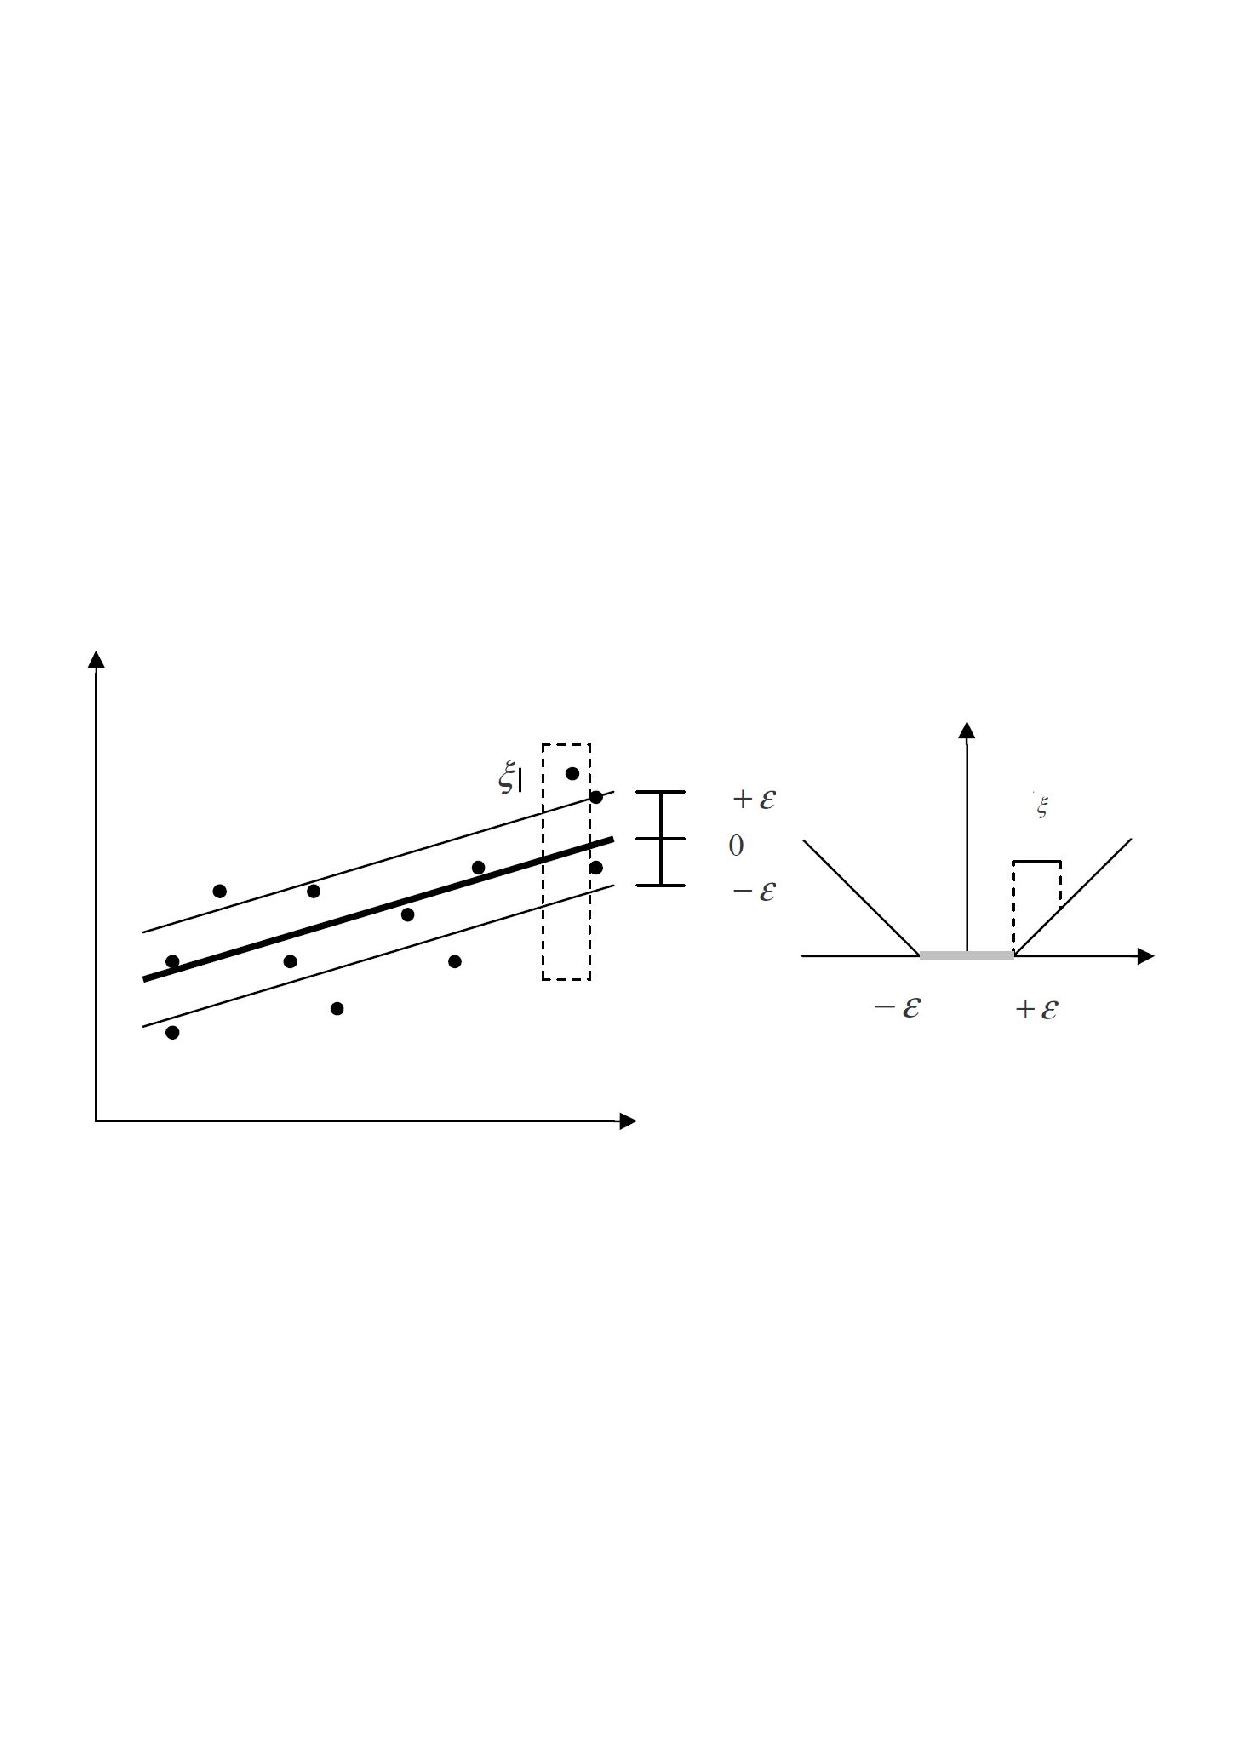
\includegraphics[ height=6.5cm, width=12cm]{figures/SVR.pdf}
        \caption{Support Vector Regression \cite{basak2007support}}
        \label{fig:single_SVR}
    \end{figure}
\bigskip
\\$1_d=[1,1,\cdots,1]^{\intercal} \in \mathbb{R}^d$ and the superscript such as $n_h$ and $d$ represents the dimension of vectors.  And $Z=[\varphi (\textbf{x}_1), \varphi (\textbf{x}_2), \cdots , \varphi (\textbf{x}_l)] \in \mathbb{R}^{n_h \times l}$ who has a inner function $\varphi$ which maps vector $\textbf{x}$ to some high Hilbert space from $d$ dimension to $n_h$ dimension. To solve the above objective function in Equation \ref{eq:obj_fun_Single_SVM}, Karush-Kuhn-Tucker (KKT) condition method is applied by assigning a Lagrange vector $\alpha = (\alpha_1, \alpha_2,\cdots,\alpha_l)^{\intercal}$ to the constraints, which contain one Lagrange multiplier for each constraint. After applying KKT condition method and some further manipulation, the objective function in Equation \ref{eq:obj_fun_Single_SVM} can be transformed into following form \cite{xu2013multi}:
\begin{align}
    \begin{bmatrix} 0 & 1_l^{\intercal} \\ 1_l^{\intercal} & X \end{bmatrix} 
    \begin{bmatrix} b \\ \alpha \end{bmatrix} &=
    \begin{bmatrix} 0  \\ y \end{bmatrix}
    \label{eq:single_SVM_solution}
\end{align}
, where $X = K + \gamma^{-1} I_{-1}$ and $K=Z^{\intercal} Z \in \mathbb{R}^{l \times l} $. The element of the $i^{th}$ row and $j^{th}$ column in matrix $K$ can be written as \cite{suykens2002least}:
\begin{align}
    K_{i,j} &= {\varphi(\mathbf{x}_i)}^{\intercal} {\varphi(\mathbf{x}_j)} 
    = \kappa({\mathbf{x}_i} \,, \mathbf{x}_j)
    \label{eq:SVM kernel func}
\end{align}
, where $\kappa({\mathbf{x}_i} \,, \mathbf{x}_j)$ represents the kernel function which shows the same result with ${\varphi(\mathbf{x}_i)}^{\intercal} {\varphi(\mathbf{x}_j)}$ under Mercer's theorem. There are several kernel functions such as Gaussian kernel, Cosine kernel, and radial basis function kernel(RBF) which is selected in this project. By utilizing the kernel function, new features are generated automatically which transform the linear model into a nonlinear model, and the new dimensions in Hilbert space are dependent on the type of the kernel function. To better solve the Equation \ref{eq:single_SVM_solution}, some reformulation is applied which is introduced in \cite{suykens2002least}:
\begin{align}
    \begin{bmatrix} s & 0_l^{\intercal} \\ 0_l^{\intercal} & X \end{bmatrix} 
    \begin{bmatrix} b \\ \alpha + b X^{-1} 1_l \end{bmatrix} &=
    \begin{bmatrix} 1_l^{\intercal} X^{-1} y   \\ y \end{bmatrix}
    \label{eq:single_SVM_solution_revised}
\end{align}
, where $s=1_l^{\intercal} X^{-1} 1_l \in \mathbb{R}_+ $ and the optimal result can be obtained for the objective function in Equation \ref{eq:obj_fun_Single_SVM} which are $\alpha^{*}$, $w^{*}$,  and $b^{*}$. By using the optimal parameters calculated above, the optimal hyper plane can be obtained and the corresponding decision function for making predictions can be built as \cite{xu2013multi}:
\begin{align}
    f_{SVR}(x) &=\langle \varphi (x) ^{\intercal}  \,,  w^{*} \rangle  + b^{*} = \sum_{i=1}^{l} \alpha_i^{*} 
                    \kappa({x_i} \,, x)+b^{*}
    \label{eq:single_SVM_pred}
\end{align}
From the above equation, it can be found that kernel function replace the inner product between the non-linear mapping variable and weight vector which allow the burden from creating non-linear mapping functions \cite{xu2013multi}.

\subsubsection{Multi-output LS-SVR}
\\To consider the correlations between outputs, Multi-output Least-square Support Vector Regression (MLS-SVR) has been developed by Xu \cite{xu2013multi}. When there are totally $m$ outputs,
to transform single-output SVR to MLS-SVR, the elements in the weight vector $w_i$ can be expressed by the sum of two vectors as follows:
\begin{align}
    w_i=w_0+v_i
\end{align}
, where $w_i \in \textbb{R}^{n_h}$ for $i \in \textbb{N_m}$ is the weight vector of the $i^{th}$ output. $w_0$ is called the mean vector which stands for the common part between each $w_i$ for $i \in \textbb{N_m}$ and $v_i$ represents the differences between each $w_i$ for $i \in \textbb{N_m}$. The mean vector $w_0$ is big when the output are similar to each other, otherwise $w_0$ is small. This way, the aim of the optimization problem is finding the optimal value of $w_0 \in \mathbb{R}^{n_h}$, $V = ( v_1, v_2, \cdots, v_m ) \in \mathbb{R}^{n_h \times m} $, and $b = (b_1, b_2, \cdots, b_m) \in \mathbb{R}^{m}$. Based on the assumptions above, the objective function of MLS-SVR can be formulated as follows \cite{xu2013multi}:
\begin{equation}
    \begin{aligned}
    & \underset{ w_0, b, V}{\text{minimize}}
    & & J( w_0, V, \Xi)= \frac{1}{2} \langle w_0^{\intercal} \,, w_0 \rangle +\frac{1}{2} \frac{\lambda}{m} \mathrm{trace} (\langle \Xi^{\intercal} \,, \Xi \rangle) \\ 
    & \text{subject to}
    & & y = \langle  Z^{\intercal} \,, W \rangle + \mathrm{repmat}(b, l, 1 )+\Xi\\
    \label{eq:obj_fun_MLS_SVM}
    \end{aligned}
\end{equation}
, where $ \Xi = ( \xi_1, \xi_2, \cdots, \xi_m ) \in \mathbb{R}^{l \times m}$ are the penalty vector for $m$ outputs, $ W = ( w_1, w_2, \cdots, w_m ) \in \mathbb{R}^{n_h \times m}$, and $\lambda, \gamma \in \mathbb{R}_{n_h}$ are two positive real regularized parameters \cite{xu2013multi}. The function $\mathrm{trace}(A)$ represents the sum of the diagonal elements in square matrix $A$ and the function $\mathrm{repmat}(A, m, n)$ create a new matrix of $m$ rows and $n$ columns whose element is $A$.
\bigskip
\\Similar with LS-SVR, the objective function above can be solved by transforming it into linear equations with the help of KKT condition method. Assuming $\alpha = ( \alpha_{1}^{\intercal}, \alpha_{2}^{\intercal},\cdots,\alpha_{m}^{\intercal} ) \in \mathbb{R}^{ml}$, where $ml = m \times l$, is the vector form of the langrange multiplier for $m$ number of constraints. The function $\mathrm{blockdiag(A_1, A_2,\cdots, A_n)}$ creates a diagonal matrix whose diagonal elements are $(A_1, A_2,\cdots, A_n)$ and the rest elements are zero. After some manipulations, the following equations can be obtained \cite{xu2013multi}:
\begin{align}
    \begin{bmatrix} 0_{ml \times m} & P^{\intercal} \\ P^{\intercal} & X \end{bmatrix} 
    \begin{bmatrix} b \\ \alpha \end{bmatrix} &=
    \begin{bmatrix} 0_m  \\ y \end{bmatrix}
    \label{eq:MLS_SVM_solution}
\end{align}
, where $P=\mathrm{blockdiag} (1_l, 1_l,\cdots, 1_l ) \in \mathbb{R} ^{ml \times m}$, $X=\Omega+ \gamma^{-1} I_{ml}+\frac{m}{\lambda} Q \in \mathbb{R} ^{ml \times ml}$, $\Omega=\mathrm{repmat}( K,m,m) \in \mathbb{R}^{m \times m}$, $K= Z^{\intercal} Z \in \mathbb{R}^{l \times l}$ and $y=(y_1^{\intercal}, y_2^{\intercal},\cdots, y_3^{\intercal}) \in \mathbb{R}^{ml}$. After solving Equation \ref{eq:MLS_SVM_solution}, the optimal value $\alpha^*$ and $b^*$ can be obtained thus the corresponding decision function is shown as follows \cite{xu2013multi}:
\begin{align}
    f_{MLS-SVR}(\mathbf{x}) &= 
     \mathrm{repmat}( \sum_{i=1}^{m} \sum_{j=1}^{l} \alpha_{i,j}^{*} 
                    \kappa({x_i} \,, x_j),1,m)+\frac{m}{\lambda} \sum_{j=1}^{l} \alpha_j^*\kappa({x_i} \,, x_j) +{b^{*}}^{\intercal}
    \label{eq:MLS_SVM_regression}
\end{align}
By utilizing the above equations, prediction can be made based on the historical data and parameter $\alpha^*, b^*$. Finally, the MLS-SVR function for prediction can be written as:
\begin{align}
    x_p &= f_{predict} (x_{train},x_{test},\alpha^*, b^*,\lambda,p)
    \label{eq:MLS_SVM_prediction}
\end{align}
, where $x_p$ is the predicted value, $x_{train}$ is the training set and $x_{test}$ is the test set. $p$ is the hyperparameter for the kernel function. $\lambda$ and $p$ can be determined by grid search method with the data in the training set \cite{xu2013multi}.
\subsubsection{SVR-EKF Algorithm}
SVR-EKF is a combined algorithm between SVR and EKF. The basic idea is to estimate the voltage magnitude of the buses based on SVR and estimate the voltage phase angle by EKF. Before estimating the state of the system based on the measurements from the smart meters, it is necessary to generate the training set for the estimation process in SVR. By setting the feeder bus to the slack bus, the voltage magnitude is $1$ $p.u$ and the voltage phase angle is $0$ $rad$ at the feeder bus. In addition, assigning active power injection and reactive power injection at each bus except the slack bus, these buses are treated as PQ buses in the power flow calculation. Assuming there are totally $n$ buses in the system, there is one slack bus and $n-1$ PQ buses, and the power flow calculation can be simulated based on the above information. After the power flow calculation, a situation where all types of measurements, including voltage magnitude, voltage phase angle, power injection at each bus, and power flow at each branch, are known and without error can be obtained.
\bigskip
\\After obtaining the full-knowledge of the system with power flow calculation, the input and output of the training set for SVR should be determined. The input for training SVR are the measurements from the training set in the full-knowledge situation, whose corresponding information in the test set are known in the real system including real meter measurements, pseudo-measurements, and virtual measurements. And the outputs of SVR are voltage magnitudes and voltage phase angle at each bus. Because the performance of SVR is heavily dependant on the training set, the training set should be updated regularly when the difference between the value of the power injections in the training set and the test set increases, such as when more households are equipped with a PV panel and the power injection at the corresponding buses increases. 
\bigskip
\\After obtaining the training set, SVR can be trained and the optimal $\alpha^*$ and $b^*$ can be obtained for predicting the voltage magnitude and phase angle at each bus by Equation \ref{eq:MLS_SVM_prediction}. In the test stage, the input data of the test set are all types of measurements collected from the distribution grid and the prediction can be made based on Equation \ref{eq:MLS_SVM_prediction} whose output are voltage magnitudes and phase angle at each bus. These predicted voltage magnitudes and phase angle by SVR are then sent to EKF firstly as the predicted state $\widetilde{x}$, which replaces the Holt's linear exponential smoothing technique in Equation \ref{eq:quasi_steady_state behaviour function}, to estimated the state of the distribution grid at time step $k+1$. After getting the predicted state $\widetilde{x}_{k+1}$ by SVR, EKF is run based on the equations introduced in Sect.~\ref{sect:EKF} except the step for calculating the state transition function $F_k$ at time step $k$ in Equation \ref{eq:quasi-transition matrix}, which is instead calculated as follows:
\begin{align}
    F_k &= \widetilde{x}_{k+1} \hat{x}_k^{-1}
    \label{eq:SVM transtion function}
\end{align}
, where $\widetilde{x}_{k+1}$ is the predicted state by SVR at time step $k+1$ and $\hat{x}_k$ is the estimated state by SVR-EKF at the $k^{th}$ time step. After the simulation of EKF, the estimated voltage phase angle $\hat{\theta}_{k+1}$ is selected as the final estimated voltage phase angle for time step $k+1$, but the estimated voltage magnitude $\hat{V}_{k+1}$ by EKF is neglected and replaced by the predicted voltage magnitude $\widetilde{V}_{k+1}$ from SVR which is the final estimated voltage magnitude due to its higher accuracy. Figure \ref{fig:flow_chart_SVR} shows the flowchart of the whole procedure of MLS-SVR voltage magnitude prediction process from training to forecasting.
    \begin{figure}[!h]
        \centering
        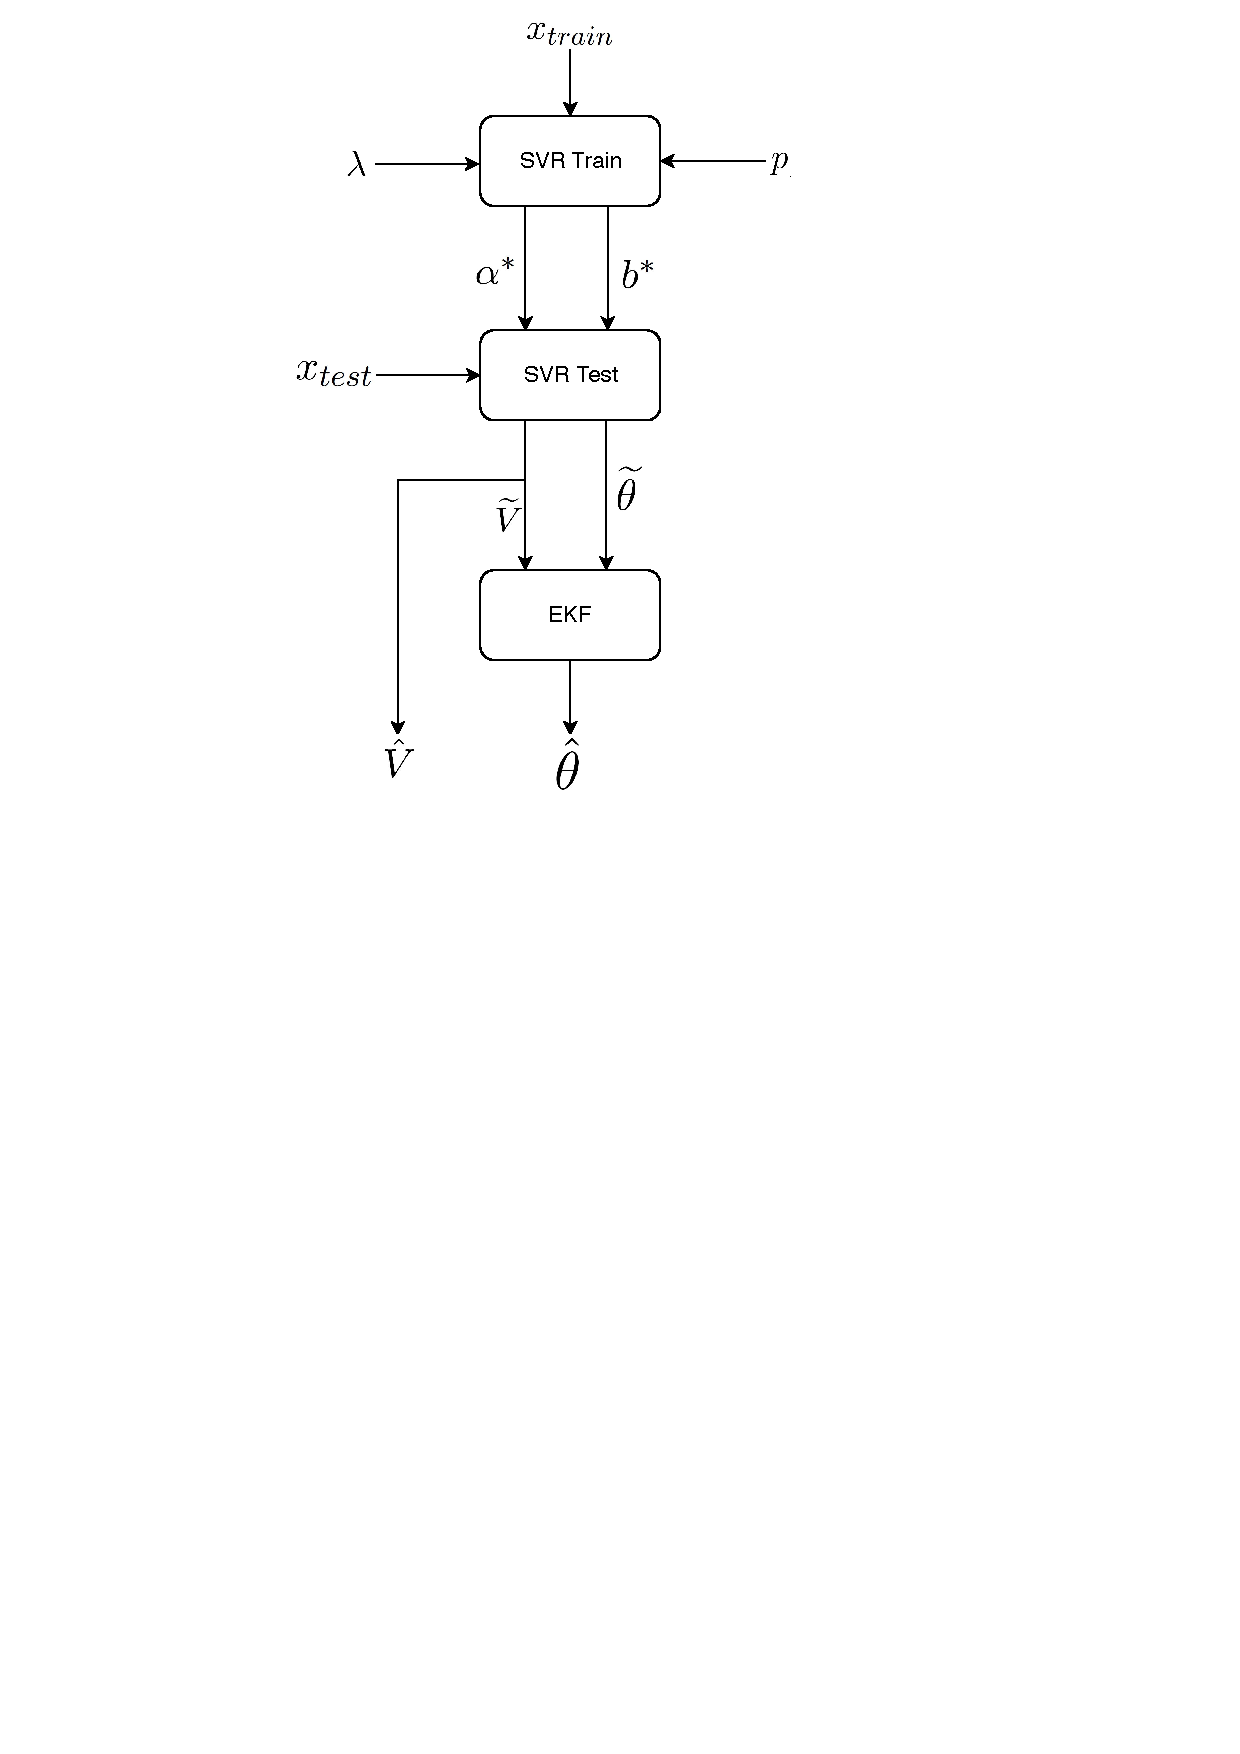
\includegraphics[ height=15cm, width=11cm]{figures/SVR_flow.pdf}
        \caption{Flowchart of SVR-EKF}
        \label{fig:flow_chart_SVR}
    \end{figure}
\bigskip
\\In conclusion, the output voltage magnitudes of SVR are used for both the prediction $\widetilde{V}$ for EKF and the final estimated voltage magnitude $\hat{V}$, whereas the output voltage phase angle of SVR are only used for the prediction stage $\widetilde{\theta}$ for EKF. The estimated voltage phases angle $\hat{\theta}$ is obtained through EKF. The reason why the predicted voltage phase angle from SVR cannot be the estimated value is because the reactive power injection in this thesis is much smaller than the active power injection, which means the voltage phase angles are close to zero and even a small estimated voltage phase error leads to a high estimated power flow error. So, the estimated voltage phase angle from EKF has a higher accuracy compared to the predicted voltage phase angle from SVR in this case.


\newpage